
\centerline{\textbf{ \LARGE Pipeline }}

\begin{enumerate}
    \item Instruction Execution \\
        \begin{figure}[h]
            \centering   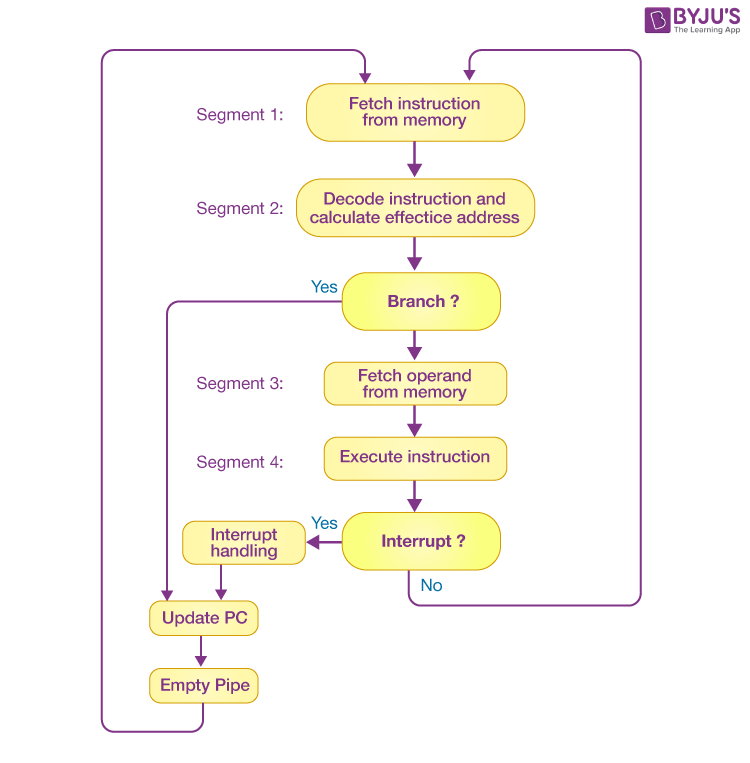
\includegraphics[scale=0.5]{./images/instruction-execution.png}
        \end{figure}

    \item To read from memory following steps are used.
    \begin{enumerate}
        \item Load MAR with address of memory where data is stored
        \item Initiate Memory Read operation.
        \item This will load MDR with the contents of memory.
    \end{enumerate}

    \item Formulas\\
    \begin{myTableStyle} \begin{tabular}{ |m{5cm}|m{3cm}|m{5cm}| } \hline
        Stages                      &  k                & \\ \hline
        instructions                &  n                & \\ \hline
        Cycle Time                  &  \(T_c\)          &  Max(StageDelay) + Buffer Delay\\ \hline
        Total Cycles(Pipeline)      &  k + (n-1)        & \(Time = P_c * T_c\) \\ \hline
        Total Cycles(Non-Pipeline)  &  n*k              & \(Time = (NP)_c * T_c\) \\ \hline
        Speed-up                    &  n*k/(k + (n-1))  & = k, n \(\gg\) k. \\ \hline
    \end{tabular} \end{myTableStyle} \vspace{0.08in}

    \newpage
    \item Micro-operations
    \begin{enumerate}
        \item operations performed on data stored in registers are called Micro-operations.
        \item Micro-operations are predetermined for each instruction.
        \item Each instruction executes a sequence of pre-defined micro-operations.
        \item Common type of micro-operation : inter-register transfer, Arithmetic operations, Logic operations
              shift operation.
    \end{enumerate}

    \item Important Registers : PC, MAR, MDR(MBR), AC, Named Registers(\(R_i\)), Pipeline Local Registers
    \item Add R1 [Mem] : R1 = R1 + [Mem] \\
    \begin{myTableStyle} \begin{tabular}{ |l|l|l|l|l| } \hline
        IF & \makecell[l]{ Instruction Decode \\ Read Operands \\from Mem and Reg}
        &execute & \makecell[l]{ MA \\ Load and \\Store}& WB   \\ \hline

        \makecell[l]{ MAR \(\leftarrow\) PC \\ Read Signal \\ Clear \large{ \( \boldsymbol R_y\)}  \\ Z \(\leftarrow\) PC + 1 }
        & \makecell[l]{ MAR \(\leftarrow\) IR[opr addr] \\ Read Signal } & Z \(\leftarrow\) MDR + \large{ \( \boldsymbol R_y\)}
        & & R1 \(\leftarrow\) Z \\ \hline

        \makecell[l]{ PC \(\leftarrow\) Z(Branch) \\ MDR is Loaded}
        & \makecell[l]{ \large{ \( \boldsymbol R_y\)} \(\leftarrow\) R1 \\ MDR is Loaded} & & & \\ \hline

        IR \(\leftarrow\) MDR & \makecell[l]{ Generate \\ Control Signals } & & & \\ \hline

    \end{tabular} \end{myTableStyle} \vspace{0.08in}

    \item Instruction Cycle.\\
    \begin{myTableStyle} \begin{tabular}{ |l|m{6cm}|m{8cm}| } \hline
        IF & \makecell[l]{ 3 Steps and 4(6) micro-operation }
           & \makecell[l]{ (1) MAR \(\leftarrow\) PC, \quad Read Signal
                            \\ \; \; \; Clear {\large \( \boldsymbol R_y\)}, \quad Z \(\leftarrow\) PC + 1
                            \\ (2) PC \(\leftarrow\) Z(Branch), \quad MDR is Loaded
                            \\ (3)  IR \(\leftarrow\) MDR }  \\ \hline

        ID & Read operands from registers and Memory
           & \makecell[l]{ (1) MAR \(\leftarrow\) IR[opr addr] \quad Read Signal
                          \\ (2) {\large \( \boldsymbol R_y\)} \(\leftarrow\) R1 \quad MDR is Loaded
                          \\ (3) Generate Control Signals } \\ \hline

        Exe & Performs ALU Oprn. Micro-operation sequence depends on opcode. Branch target is calculated
            & Z \(\leftarrow\) MDR + {\large \( \boldsymbol R_y\)}  \\ \hline

        MA & Load and Store instructions & \makecell[l]{ (1) LOAD : Z \(\leftarrow\) [Mem]
                                           \\ (2) STORE: [Mem] \(\leftarrow\) Z } \\ \hline

        WB & Write result in Register &  {\large \( \boldsymbol R_i\)}\(\leftarrow\) Z \\ \hline
    \end{tabular} \end{myTableStyle} \vspace{0.08in}


    \begin{minipage}{\linewidth}
    \item Structural Hazards.
    \begin{enumerate}
        \item Hardware resource conflicts among the instructions in the pipelin.
        \item Memory, a GPR Register, or an ALU
        \item Fetch cycle and Execution cycle both may need ALU at the same time. Fetching involves calculating Effective Address.
        \item more than one instruction in the pipe requires access to the very same resource in the same clock cycle.
        \item Solution: Introduce bubble
        \item Solution: Separate memory for Instruction and Data.
        \item Solution: Use of register files. Allows access to one write register, and one read register.
    \end{enumerate}

    \item Data Hazards : RAW, WAR, WAW.
    \begin{enumerate}
        \item instruction is dependent on the results of a previous instruction.
        \item Bernstein condition.
        \item Solution: Re-order instruction by compiler.
        \item Solution: Introduce bubble or NOP instruction.
        \item Solution: Data forwarding sends data directly to the desired pipeline unit.
        \begin{enumerate}
            \item dependent instruction access registe's new value from the pipeline interface register directly.
            \item Operand Forwarding can avoid stalls only if the dependent instructions are ALU type instructions
        \end{enumerate}
    \end{enumerate}

    \item Control Hazards
    \begin{enumerate}
        \item caused by branch instructions.
        \item Result of instruction determines the next instruction to be executed.
        \item Solution: Re-order instruction. The Compiler is used to implement this delayed branch.
        \item Solution: Introduce bubble(Stalling).
        \item Solution: Prediction.
        \item Solution: Dynamic Branch Prediction : Branch Table Buffer
        \item Branch penalty = total no of stalls.
        \item If the target address is present after the kth stage, then there will be (k – 1) stalls.
        \item Total number of stalls = Branch frequency * Branch Penalty
    \end{enumerate}
    \end{minipage}

    \item  Control unit in a pipelined design

\end{enumerate}
